\chapter{La Composition des services web}
%% TODO Introduire la notion de la composition et le plan du chapitre

%   % Dans le chapitres précédent, nous avons étudiés la description, la
% publication,  la découverte et la sélection de services Web
% élémentaire. L'autre concept fondamentale % est la composition des
% services web.


  
%   % The other fundamental concept is web service composition which
% sometimes overlaps or will merge with the process of WS
% discovery. WS composition is a mechanism of combining two or more
% basic services into a possibly complex service. It is used to solve
% complex problems by combining available basic services. It helps to
% accelerate rapid application development and facilitate service
% reuse from developer perspective % and from user perspective it
% increases complex service consumption. As mentioned earlier a
% composite service can be regarded as a combination of services invoked
% in % a predefined order and executed as a whole and that has more
% functionality than its components. WS composition is needed because
% finding a right service provider for the request is not an easy task
% on fast growing WWW sometimes it is even % impossible. Thus WS
% composition becomes necessary and inevitable. Composing WS from
% existing ones is an effective method to fill this gap.\cite{Omer2011}

%   Dans ce chapitre, nous présentons dans un premier temps les
% définitions et les types de composition de services Web présents dans
% la littérature. Ensuite, nous étudions .....
%   Enfin, un ensemble de travaux proposent des approches de la
% composition dynamiques des services web sémantiques.
  

\newpage

  \section{Définition et types de composition}
  \label{sec:defin-et-caract}

  Cette section a pour but d'exposer, d'une part, quelques définitions
  et objectifs de la composition des services Web proposées par la
  communauté, et d'autre part, les différents types et mécanismes de
  composition selon différents points de vue rencontrés dans la
  littérature.
  
  \subsection{Définitions}
    \label{sec:definitions}

    Martin \emph{et al.} \cite{martin2004owl} définissent
    la composition comme étant \emph{``le processus de sélection, de
      combinaison et d'exécution de services en vue
      d'accomplir un objectif donné''}.\\
  
    Selon S. Dustdar et W. Schreiner \cite{dustdar2005survey} :
    \emph{`` L'infrastructure de base des services Web suffit pour la
      mise en œuvre d'interactions simples entre un client et un
      service Web. Si la mise en œuvre d'une application métier
      implique l'invocation d'autres services web, il est nécessaire
      donc de combiner les fonctionnalités de plusieurs services
      web. Dans ce cas, nous parlons d'une composition de services
      Web''}.\\
    
    En d'autre terme, La composition de services Web désigne une
    opération qui consiste à construire de nouvelles applications ou
    services appelés \textbf{services composites} ou agrégats par
    l'assemblage ou l'agrégation de services existants nommés
    \textbf{services atomiques} ou
    élémentaires.\\

    Il existent différentes techniques de composition de services web
    développées par la littérature. ces techniques sont également
    classés en fonction de différents critères.

    Selon les travaux, les définitions des types de composition
    diffèrent d'une communauté de l'autre.

    Barros \emph{et al.} \cite{barros2006standards} classent la
    composition des services Web en trois catégories: orchestration,
    chorégraphie et comportementale.

    \cite{peltz2003web} de ça part distingue deux ...
    %% commment classifies la compositions ?
    %% \cite{fluegge2006challenges} Static vs dynamique.

    %% Les Procédés de coordination comme une vision (point de vue)
    %% d'une composition des services Web.

    % TODO: vertical vs horiontal composition selon
    % medjahed.\cite{medjahed2004thesis}

      \subsection{Procédés de coordination}
      \label{sec:proc-de-coord}

      %% Introduire la notion d'un procédé de coordination
      Selon Peltz \cite{peltz2003web}, Nous distinguons deux
      catégories de procédés de coordination utilisés pour décrire la
      composition de services dans un flot de processus métier. des
      procédés implémentant l'\emph{orchestration} de services et des
      procédés implémentant la \emph{chorégraphie} des services.

      % ces termes (\textit{orchestration} et \textit{chorégraphie})
      % décrivent deux aspects de création des processus métiers à
      % partir des services Web composites \cite{peltz2003web}.

      \begin{figure}[h]
    \centering
    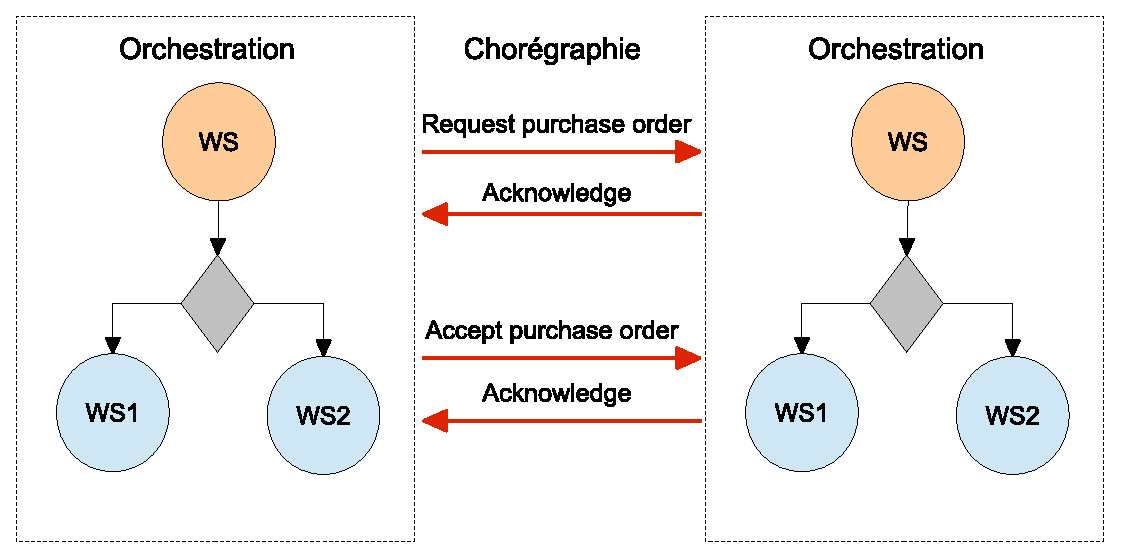
\includegraphics[width=1\textwidth]{figs/orchestration-vs-choregraphie.eps}
    \caption{Orchestration vs Chorégraphie selon Peltz
      \cite{peltz2003web}.}
    \label{fig:orchestration-vs-choregraphie}
\end{figure}

      \textbf{Un procédé} est représenté par un graphe orienté
      d'activités ou un flot de contrôle qui donne l'ordre d'exécution
      des activités et la logique de coordination des services. Chaque
      activité représente une fonctionnalité réalisée concrètement par
      un service \cite{chollet2009orchestration}. La figure
      \ref{fig:orchestration-vs-choregraphie} illustre ces deux
      approches en conjonction.
      % a figure orchestration vs chorégraphie

      % It should be noted that these models are not used exclusively:
      % one approach can implement more than one models at the same
      % time.\cite{baryannis2010} %% TODO: translate

        \subsubsection{Orchestration}
        \label{sec:orchestration}
        % Selon Sanlaville \cite{jamal2005environnement} : \emph{``
        %   L'orchestration des services Web permet de définir
        %   l'arranegement et l'enchaînement de ces services selon un
        %   canevas bien défini. Elle décrit la manière par laquelle les
        %   services peuvent interagir ensemble tout en incluant l'ordre
        %   d'exécution des différentes interactions''}.
        Barros \emph{et al.} \cite{barros2006standards} définissent
        l'orchestration comme un ensemble de processus exécutés dans
        un ordre prédéfini afin de répondre à un but
        \cite{lopez2008selection}. Ce type de composition se base sur
        un procédé métier exécutable permettant de décrire
        d'enchaînement et les interactions des différents services
        basiques collaborant dans une composition.

        L'orchestration offre \textbf{une vision centralisée} de
        contrôle, le procédé est toujours contrôlé par l'un des
        partenaires métiers. Ce dernier joue le rôle d'un chef
        d'orchestre qui se charge d'appeler les services de la
        composition suivant l'ordre d'exécution déjà défini par le
        processus métier.

        Le principe de l'orchestration est illustré
        par La figure \ref{fig:orchestration}.

        \begin{figure}[h]
    \centering
    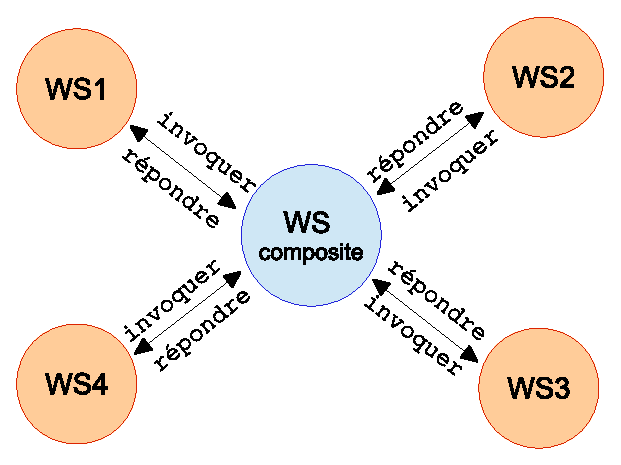
\includegraphics[width=0.6\textwidth]{figs/orchestration.eps}
    \caption{Principe de l’orchestration des services Web.}
    \label{fig:orchestration}
\end{figure}

        \subsubsection{Chorégraphie}
        \label{sec:choregraphie}
        % Selon Sanlaville \cite{jamal2005environnement} : \emph{`` La
        %   chorégraphie permet de tracer la séquence de messages
        %   échangés dans un contexte de composition de services
        %   Web. Elle est typiquement liée à la description de
        %   conversations existantes entre les services tout en
        %   impliquant plusieurs parties, incluant les clients, les
        %   fournisseurs et les partenaires''}.

        D'après Barros \emph{et al.} \cite{barros2006standards}, la
        chorégraphie permet de décrire la composition comme un moyen
        d'atteindre un but commun en utilisant un ensemble de services
        Web. La collaboration entre chaque service Web de la
        collection (faisant partie de la composition) est décrite par
        des flots de contrôle \cite{lopez2008selection}.

        La chorégraphie exprime une vue d'ensemble des services
        interagissant dans le cadre d'une composition de
        services. Selon Peltz \cite{peltz2003web}, la chorégraphie
        illustre les différants échanges de messages entre les
        participants. la chorégraphie offre \textbf{une vision
          décentralisée} et globale.

        Le principe de la chorégraphie est illustré par la figure
        \ref{fig:choregraphie}.
        % TODO : redraw the fig
        \begin{figure}[h]
    \centering
    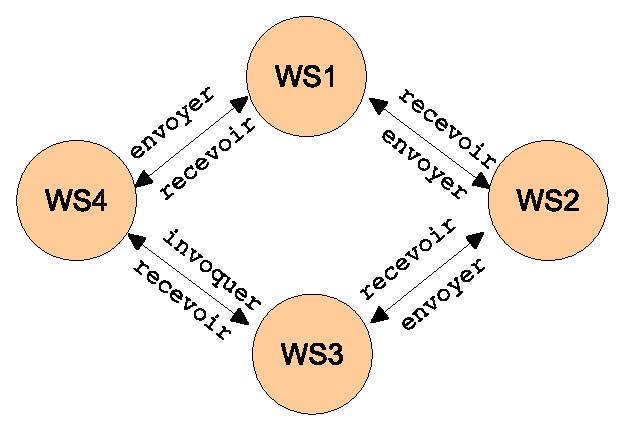
\includegraphics[width=0.6\textwidth]{figs/choregraphie.eps}
    \caption{Principe de la chorégraphie des services Web.}
    \label{fig:choregraphie}
\end{figure}


      \subsection{Types de composition}
      \label{sec:types-de-composition}
      Selon \cite{fluegge2006challenges}.

      % La composition des services Web peut être soit une composition
      % statique soit une e composition dynamique:

      % – La composition statique : est appelée aussi composition
      % off-line, précompilée ou encore proactive. C'est une composition
      % qui utilise des services basiques qui sont au préalablement
      % définis d' une façon figée et qui ne peuvent pas changer en
      % fonction du contexte du client. Ce type de composition engendre
      % des applications peu flexibles, parfois inappropriées avec les
      % exigences des clients.

      % – La composition dynamique : appelée aussi composition on-line,
      % postcompilée ou encore réactive. Elle se réfère à la sélection
      % des services basiques à la volée. Autrement dit, la sélection
      % des services basiques ne peut pas être prédéfinie à l'avance
      % mais elle sera faite au moment de l'exécution en fonction des
      % contraintes e imposées par le client. Ceci permet d' élaborer
      % différents scénario de composition qui offrent les mêmes
      % fonctionnalités et qui tiennent compte de la dynamique de la
      % situation du client.


      % Microsoft Biztalk et Bea WebLogic sont deux exemples de moteurs
      % de composition statiques de services Web. Pour la composition
      % dynamique, nous trouvons les plate-formes e-flow de HP et Sword
      % de Stanford.

      % Dans le cadre d'une composition statique de services, si les
      % fournisseurs proposent d'autres services ou changent les anciens
      % services, des incohérences peuvent être causées. Ceci qui
      % demande un changement de l'architecture du logiciel, voire de la
      % définition de l'application et crée l'obligation de faire une
      % nouvelle conception de l'application. C'est pourquoi, la
      % composition statique des services web est considérée rigide et
      % trop ee restrictive [86 S. Sanlaville, Environnement de proc ́d ́
      % extensible pour l'orchestration : Application aux services e e
      % web, Ph.D. Thesis, 2005 ]
      % \cite{driss2011approche}

        \subsubsection{Composition manual/automatique}
        \label{sec:comp-manu}

        \subsubsection{Composition statique/dynamique}
        \label{sec:comp-stat}

        % La composition automatique (dynamique par le terme de
        % \cite{fluegge2006challenges} permet un développement plus
        % rapide des applications à base de services. Elle consiste à
        % préciser la requête d'un utilisateur sous forme d'objectifs à
        % satisfaire. Un moteur de composition \textit{``intelligent''}
        % choisit la comabinaison de services répondant à l'objectif
        % décrit. Il génère la composition de service adéquate de
        % manière transparente à l'utilisateur. Ce principe a interpellé
        % plusieurs communautés de recherche travaillant dans le domaine
        % de l'Intelligence Artificielle.
        % \cite{elie2010}


      % La composition requiert la description et l'organisation de
      % l'interaction entre les services. Elle nécessite la gestion de
      % plusieurs aspects comme les échanges de données entre les
      % services, les pannes ou erreurs éventuelles, le contexte
      % d'interaction, le degré d'automatisation des tâches, etc. Dans
      % la littérature, une variété de spécifications, de langages et
      % d'approches formelles ont étudiés la composition.

      % Dans la suite nous présentons les deux approches principales de
      % description de la composition en section
      \ref{sec:lang-de-comp}...
      \newpage

  \section{Languages de composition des services web}
  \label{sec:lang-de-comp}
  %% TODO: an introduction to the section
  Afin de supporter la composition de services, plusieurs langages de
  composition de services ont été proposés comme ...

  Dan cette section on va détiller trois languages ...
  %% \cite{lopez2008selection}

    \subsection{BPEL}
    \label{sec:bpel}

    \acrshort{bpel} est une spécification du consortium OASIS
    \footnote{\url{https://www.oasis-open.org}}issue de la fusion des
    spécifications \acrshort{xlang} Microsoft
    \footnote{\url{http://www.microsoft.com}}et \acrshort{wsfl} d'IBM
    \footnote{\url{http://www.ibm.com}}, il hérite les
    caractéristiques d'un langage structuré en blocs de
    \textsc{XLANG}, ainsi que les caractéristiques d'un graphe direct
    de WSFL \cite{driss2011approche}.

    \begin{figure}[h]
    \centering
    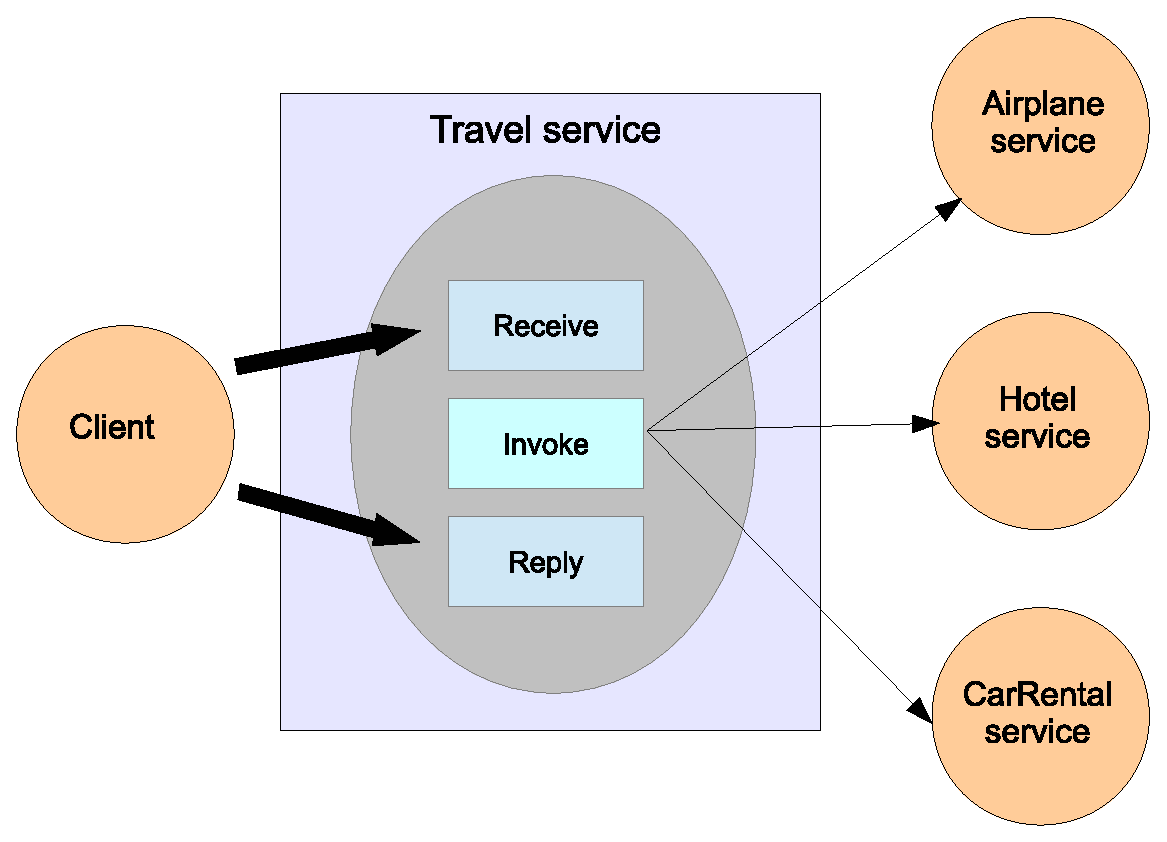
\includegraphics[width=0.8\textwidth]{figs/bpel-travel-example-shema.eps}
    % TODO translate the figure
    % TODO reference the fig
    \caption{Une vue interne de service de voyage \textsc{bpel}.}
    \label{fig:3w_to_sws}
\end{figure}
%%% Local Variables: 
%%% mode: latex
%%% TeX-master: "3w_to_sws"
%%% End: 

    \begin{figure}[h]
    \centering
    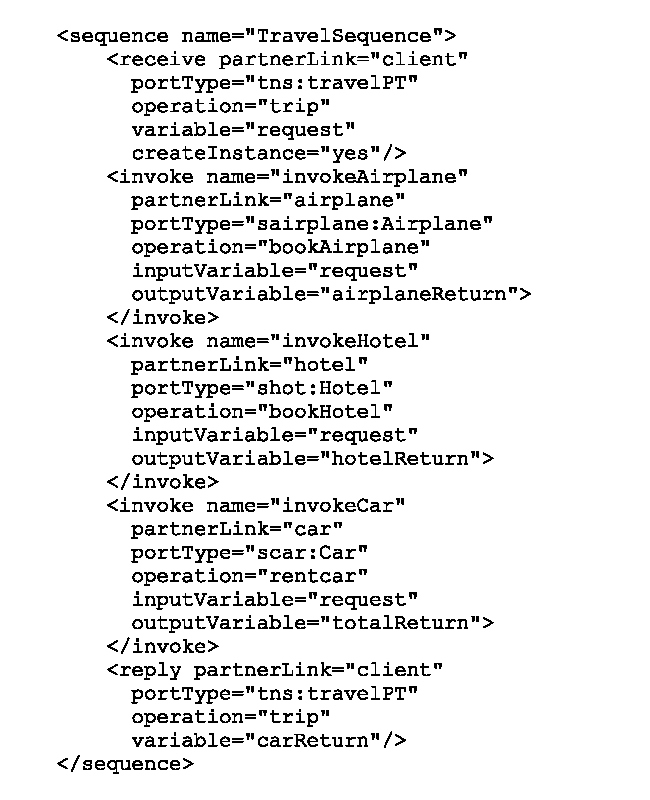
\includegraphics[width=0.8\textwidth]{figs/bpel_travel_example_document.eps}
    % TODO translate the figure
    % TODO reference the fig
    \caption{Le procédé d'orchestration de service de voyage \textsc{bpel}.}
    \label{fig:bpel_travel_example_document}
\end{figure}


    \textsc{BPEL} \textit{(appelé aussi \acrshort{bpel4ws} ou
      \acrshort{ws-bpel})} est le langauge d'\textbf{orchestration}
    le plus utilisé dans l'industrie permettant la coordination des
    interactions entre l'instance du service composite et ses
    partenaires sous forme d'un schéma \acrshort{xml} \textit{(le
      scriprt d'orchestration)}, il définit le processus,
    l'enchaînement et l'ordonnancement des actions qui seront
    exécutées par le moteur d'orchestration, agissant comme une
    machine virtuelle capable d'exécuter \textbf{le procédé métier}
    intéreptable de \textbf{coordination}
    \cite{chollet2009orchestration}.
    % TODO: BPEL permet de quoi ? et comment ?

    % Un procédé est composé d'activités qui s'enchaînent grâce à des
    % échanges de données. Les activités peuvent être de deux types:
    % basiques ou complexes. Les activités basiques sont des types de
    % base comme invoke pour appeler un service Web, receive pour
    % attendre une invocation, reply pour une réponse... A partir de ces
    % types de base, il est possible de créer des activités composites
    % avec des structures de construction du contrôle du flot de données
    % : flow pour une ou plusieurs activités concurrentes, sequence pour
    % une séquence d’activités, switch pour des conditions, while pour
    % une boucle... , \cite{chollet2009orchestration}.


    %  BPEL4WS repose sur un modle constitué d'activités de coordination
    %  qui peuvent être de deux types : de base ou structurées. Les
    %  activités de base permettent :
    %  – d'invoquer une opération d'un service Web (invoke)
    %  – de recevoir une requête (receive)
    %  – de générer une réponse a une requête (reply) ;
    %  – de copier une donnée (assign) ;
    %  – de marquer un temps d'attente (wait) ;
    %  – de terminer une activité (terminate).

    %  Chaque activité de base est réalisée par une opération d'un
    %  service et chaque service est associé à un
    %  PartnerLink. Celui-ci contient les informations sur le rôle
    %  et l'interface PortType du service qui réalise cette opération.
    %  Les activités structurées utilisent les activités de base pour
    %  décrire :

    %  – des séquences ordonnées (sequence) ;
    %  – des exécutions en parallèle (flow) ;
    %  – des branchements conditionnels (switch,if) ;
    %  – des boucles (while) ; – des chemins alternatifs (pick );
    %  – des regroupements d’activités (scope).
    % \\cite{} ite{driss2011approche}

    %% procédé abstraite vs exécutable Selon \cite{chollet2009orchestration}
    % WS-BPEL est un langage de procédés basé sur la technologie XML,
    % tout comme les autres standards des services Web. WS-BPEL permet
    % de construire des procédés interprétables et exécutables par un
    % moteur d'orchestration.

    % Les procédés peuvent être modélisés de deux manières :
    % – abstraite : seuls les échanges de messages entre les
    % différents participants sont spécifiés. Mais le comportement
    % interne de ces participants n'est pas explicité.
    % – exécutable : les activités du procédé sont ordonnées; les
    % partenaires impliqués sont identifiés ainsi que les messages
    % qui sont échangés. A ceci s'ajoute le traitement des fautes
    % et des exceptions pour les cas d'erreurs.

    % TODO: an example d'un shémas BPEL
    % draw the figure [ Internal view of Travel Service (BPEL4WS)]
    % TODO: référencer ce example [Semantic web processes and their
    % application - chapter 8 (in the ch2 folder)]

  %   <sequence name="TravelSequence">
  %     <receive partnerLink="client"
  %       portType="tns:travelPT"
  %       operation="trip"
  %       variable="request"
  %       createInstance="yes"/>
  %     <invoke name="invokeAirplane"
  %       partnerLink="airplane"
  %       portType="sairplane:Airplane"
  %       operation="bookAirplane"
  %       inputVariable="request"
  %       outputVariable="airplaneReturn">
  %     </invoke>
  %     <invoke name="invokeHotel"
  %       partnerLink="hotel"
  %       portType="shot:Hotel"
  %       operation="bookHotel"
  %       inputVariable="request"
  %       outputVariable="hotelReturn">
  %     </invoke>
  %     <invoke name="invokeCar"
  %       partnerLink="car"
  %       portType="scar:Car"
  %       operation="rentcar"
  %       inputVariable="request"
  %       outputVariable="totalReturn">
  %     </invoke>
  %     <reply partnerLink="client"
  %       portType="tns:travelPT"
  %       operation="trip"
  %       variable="carReturn"/>
  % </sequence>


    % inclut la sémantique ?
    % TODO: avantages et inconvénient

    \subsection{WS-CDL}
    \label{WS-CDL}
    % make a reference to [TODO: Kavantzas et al., 2005] selon
    % elie2010
    \acrshort{ws-cdl} est un langage de composition de services de
    type \textbf{chorégraphie} qui permet de décrire une vision
    \textbf{globale} des collaborations entre les services Web
    \cite{elie2010}, à l'instar des standards de services Web,
    \textsc{WS-CDL} est basé sur \textsc{XML}, il complète la
    description \acrshort{wsdl} des services Web afin de décrire les
    interactions entre les participants (les services Web) de la
    composition.

    \textsc{WS-CDL} reprend et développe la spécification
    \acrshort{wsci} décrivant les séquences ordonnées de messages
    impliquant plusieurs entités (services Web) engagés dans une
    composition visant à accomplir un objectif commun.

    \textsc{WS-CDL} consiste à définir un fichier XML décrivant une
    chorégraphie, il permet de \cite{elie2010}:
    \begin{itemize} % WSDL-S elements and attributs
    \item désigner les variables et les types de données échangées.
    \item décrire les  activités impliquées.
    \item décrire les structures illustrant les interactions entre
      les activités.
    \end{itemize}

    %       En résumé WS-CDL permet de décrire les règles selon
    %       lesquelles une collaboration doit avoir lieu. Il fournit une
    %       structuration globale de l'interaction en fonction de
    %       laquelle chaque participant décrit son processus métier et
    %       par suite ses services.
    %  \cite{elie2010}

    %  WS-CDL (Web Service Choreography Description Language) est un
    %  langage issu des efforts de standardisation
    %  du groupe de travail du W3C portant sur la chorégraphie de
    %  services Web (Web Services Choreography Working
    %  Group52). L'objectif de ce langage est de décrire les relations
    %  entre les services Web lors d'une composition de type
    %  chorégraphie.

    %  WS-CDL est un langage de composition de services de type
    %  chorégraphie définissant des contrats multi-parties. L’avantage
    %  de ce langage est que la description des interactions (l’élément
    %  Choreography du Package) est réutilisable. Ceci permet de
    %  diminuer la charge de travail des concepteurs. L’inconvénient de
    %  WS-CDL est que même si l’élément Choreography est réutilisable,
    %  sa description reste lourde. Un service doit posséder autant de
    %  Package que de participations à des compositions. De plus, WS-CDL
    %  n’inclut pas pour le moment de sémantique. Des travaux, tels que
    %  [Kang et al., 2007a] et [Kang et al., 2007b], proposent d’étendre
    %  WS-CDL afin d’y intégrer de nouveaux concepts (tels que la
    %  gestion des erreurs et des exceptions ou la mise en œuvre d’un
    %  minuteur d’exécution de la composition).

     % \cite{lopez2008selection}

    % TODO: shémas exemple d'un document WS-CDL.
    % inclut la sémantique ?
    % TODO: avantages et inconvénients.


    \subsection{OWL-S}
    \label{sec:owl-s}
    \cite{mcilraith2003bringing}
    % see the BPEL reference for a complete schema and example

  \section{Compostion dynamique des services web}
  \label{sec:comp-dynam}

    \subsection{Techniques de planification}
    \cite{bartalos2011effective}
    \label{sec:techn-de-plan}

  % conclusion
  Introduire la composition dynamique basé sur le modle graphe qui se
  sera détaillé dans le prochain chapitre.
  \section{Conclusion}
  \label{sec:conclusion}
 

%%% Local Variables: 
%%% mode: latex
%%% TeX-master: "../main"
%%% End: